\chapter{Social Connectedness Index}
\section{Introduction}
The Social Connectedness Index (SCI) is a metric used to evaluate the strength of social connections between locations. To calculate this index, we rely on a snapshot of Facebook user networks and their interactions with friends. Locations are assigned to users based on information from their Facebook profiles, including self-reported locations as well as data derived from their device and network connections. The SCI for two locations, i and j, is defined as \cite{facebookSocialConnectedness}:
$$SocialConnectednessIndex_{i,j}=\dfrac{FB\_Connections_{i,j}}{FB\_Users_i*FB\_Users_j}$$ 
Where:
\begin{itemize}
    \item $FB\_Users_i$ and $FB\_Users_j$ represent the number of Facebook users in positions $i$ and $j$, respectively.
    \item $FB\_Connections_{i,j}$ denotes the number of connections between positions $i$ and $j$. 
\end{itemize}

The Social Connectedness Index (SCI) is a measure of the relative probability that a Facebook user in location $i$ is friends with a user in location $j$. Higher values indicate a stronger likelihood of connections between two locations, reflecting underlying social, economic, and demographic ties.

One key question in analyzing social connectedness is how the strength of these connections varies with geographic distance. Intuitively, friendships tend to be more frequent between closer locations, but the exact nature of this decline can provide insights into regional cohesion, migration patterns, and economic integration. \cite{Bailey2018}. A useful concept for quantifying this relationship is \textit{elasticity}, defined as:

$$Elasticity = \dfrac{\% Change in Friendship Links}{\%Change in DistanceElasticity}$$$

This captures how quickly social connectedness decays with distance.

Beyond elasticity, I will also explore key network properties that characterize social connectedness. In particular, I will analyze the \textit{strength distribution}, as well as \textit{strength centrality}, which identifies the most socially integrated counties based on their total connection weight. Additionally, I will examine the \textit{modularity} of the network to assess the presence of distinct clusters of highly connected regions. These structural metrics will provide a broader perspective on the patterns of social connectivity, complementing the elasticity analysis by highlighting variations in the strength and organization of social ties.

\section{Data analysis}

During the initial data preparation, the county-level SCI dataset from The Humanitarian Data Exchange \cite{HUMDataSocialConnectedness} was enhanced by adding county and state names as well as latitude and longitude coordinates. These modifications facilitated a more detailed spatial analysis of SCI flows.

To visualize these flows, I generated maps where each county is represented as a node (colored dot) labeled with its FIPS code, and edges connecting counties are scaled by the SCI weight. For instance, in Figure \ref{fig:sci_map}, the SCI flows in North Dakota are depicted; here, edge thickness is normalized to the highest SCI value to ensure even the weakest connections remain visible.

\begin{figure}[h]
    \centering
    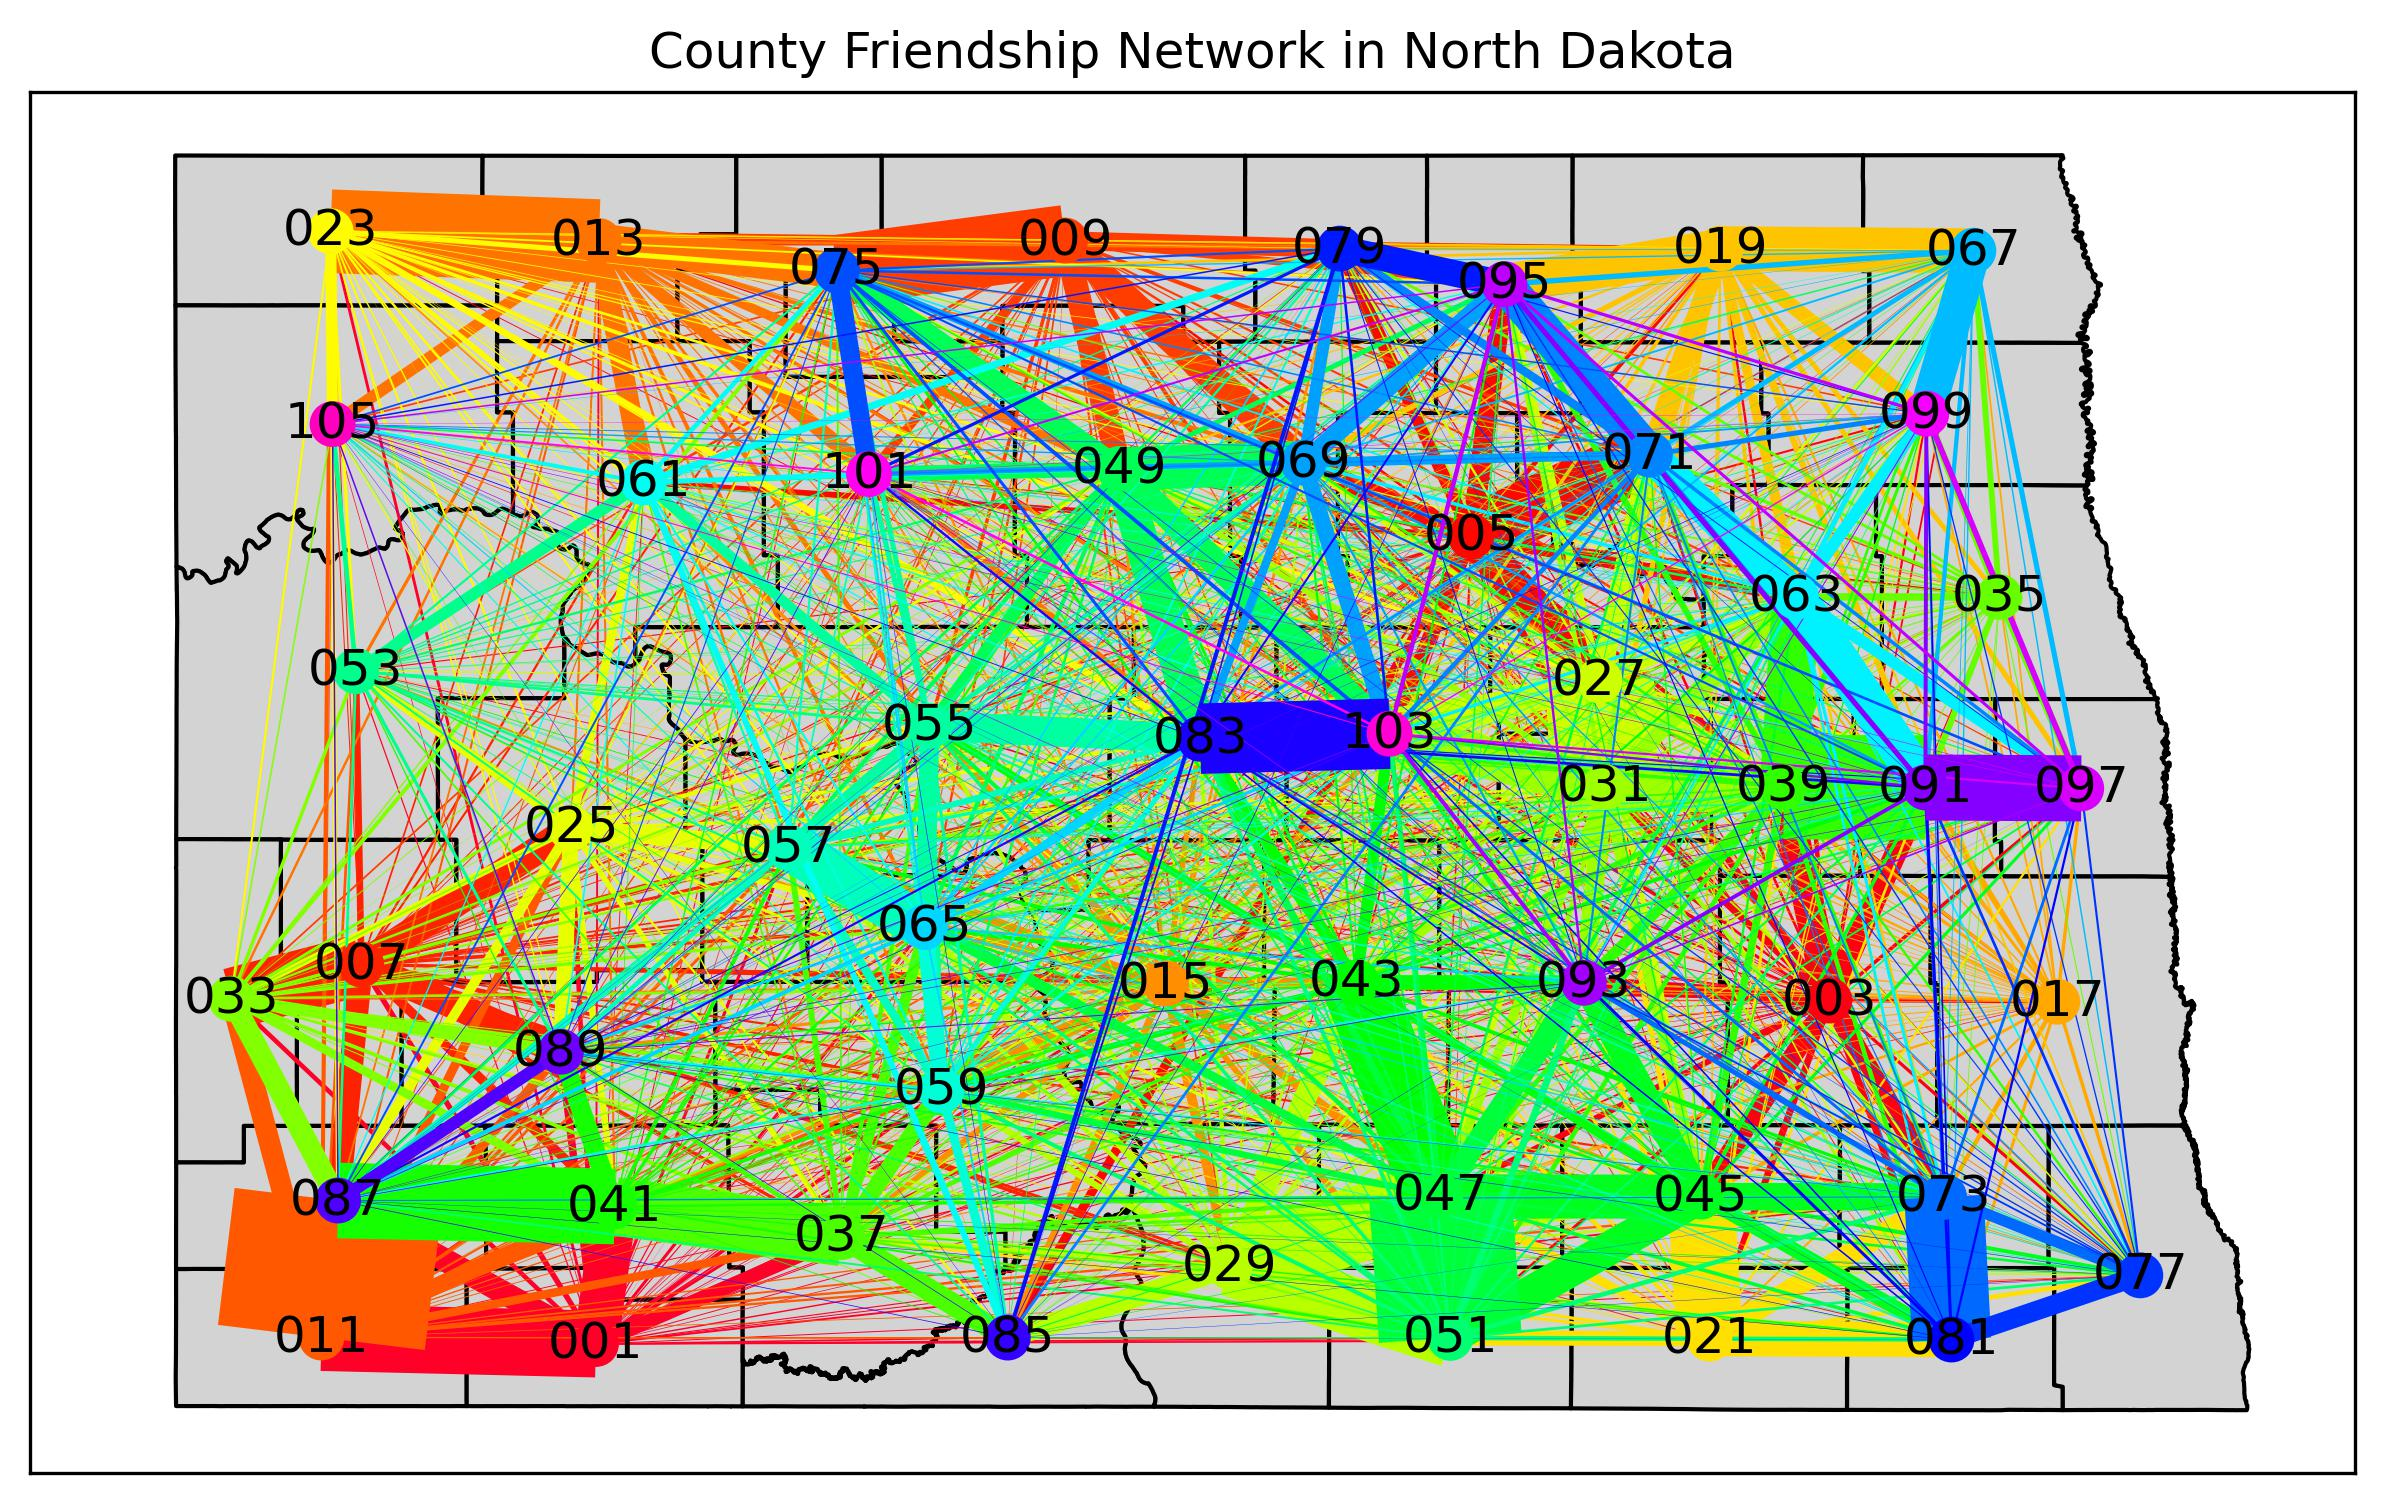
\includegraphics[width=0.8\textwidth]{images/network_North Dakota.jpg}
    \caption{County-level SCI flows in North Dakota. Nodes (colored dots) represent counties (labeled with FIPS codes) and edge thickness is proportional to the SCI weight, normalized to the maximum value.}
    \label{fig:sci_map}
\end{figure}

Subsequent analysis examined how both geographical features and migration patterns affect social connectedness. In areas like Philadelphia and surrounding states, counties within the Appalachian Mountains tend to exhibit higher SCI values, indicating stronger local connections. In contrast, in Florida, SCI maps reveal lower local connectivity, likely reflecting migration patterns in which residents maintain ties with more distant northern regions \cite{NairAndris2024}.

Table \ref{tab:elasticity_comparison} compares my elasticity estimates with those reported by Bailey et al. The results indicate that elasticity is more negative for shorter distances—implying a sharper decline in social ties with increasing separation—and becomes less negative as the distance grows. This suggests that while geographic distance is a significant factor in determining friendship links, its impact diminishes over larger scales \cite{Bailey2018}.

\begin{table}[h]
    \centering
    \begin{tabular}{lcc}
        \hline
        Distance Range & My Results & Bailey et al. \\ 
        \hline
        Full dataset & $-1.63 \pm 0.03$ & -- \\ 
        $< 200$ miles & $-1.92 \pm 0.07$ & $-1.99$ \\ 
        $\geq 200$ miles & $-1.11 \pm 0.27$ & $-1.16$ \\ 
        \hline
    \end{tabular}
    \caption{Comparison of elasticity estimates. A more negative elasticity indicates a steeper decline in social connectedness with increasing distance.}
    \label{tab:elasticity_comparison}
\end{table}

Finally, community detection was performed using the Louvain algorithm. When these communities were superimposed on topographical maps, notable spatial patterns emerged. In Montana, for example, the Louvain method identified five distinct modules. Particularly striking were two modules: one encompassing counties north of the Missouri River, and another covering regions within the Rocky Mountains. This spatial differentiation highlights the role of natural features —such as rivers and mountain ranges— in segmenting social connectivity and structuring local networks.

These preliminary findings point toward a promising direction for further research. Incorporating additional layers of data—such as migration trends, trade flows, and socioeconomic indicators—could enrich our understanding of how social connectedness is influenced by both natural and socio-economic factors, as demonstrated in the Bailey paper. 

Additionally, the correlation analysis between total population and strength centrality of SCI across different states suggests that population size alone is not a strong determinant of centrality, with correlation coefficients mostly ranging between $-0.1$ and $-0.35$. This weak negative relationship implies that other structural factors, such as geographic distribution, connectivity, and economic interactions, may play a more significant role in shaping social ties than sheer population numbers. 

Future research could incorporate additional regional characteristics to better capture the complexities of social connectivity and its underlying determinants.


\emph{
Structure as\footnote{Remove this part from the report}:
\begin{itemize}
\item A short (max 1 page) explanation of the task, including references. Include mathematical concepts.
\item Max 2 pages for the whole task (including figures)
\item It is possible to use appendices for supplementary material, at the end of the report. Max 5 pages per task
\end{itemize}
A total of 3 pages + 5 supplementary pages per task
}

\newpage